\documentclass[10pt, journal]{IEEEtran}
\usepackage{graphicx}
\usepackage{cite}

\title{DSP Processing of uFluidics Signal}
\author{Michael Nolan}
\begin{document}
\maketitle \par
Because the uFluidics device generates an extremely weak signal, when
the signal reaches the circuit to count the cells, it will have quite
a lot of noise in it. In order to accurately count the cells, the
signal will need to be processed in order to remove the noise and
detect when a cell passes through the device.

\section{DSP}
The DSP for this project needed to 
\begin{itemize}
\item Have a low cost
\item Have an on board ADC
\item Be more than able to process a 5ks/s signal (to allow for changes to processing algorithm)
\item Have enough ram to process the above signal in batches of 1024 samples
\item Be capable of driving a display or other peripherals to present results
\end{itemize}

After some searching, a dsPIC33f was determined to be able to fufill
the above requirements, and the dsPIC33FJ128GP802 was selected as it
had more than enough ram and processing power for our
use. Additionally, a less powerful DSP from the same product line
could be used in the final product after determining exactly how much
ram and processing power are needed

\section{Processing}

According to \cite{dspguide}, the optimal way to separate a known
signal from white noise is to use correlation. Via COMSOL simulation
and via a crude prototype involving dropping a straw through a coil,
the signal of interest would have a shape similar to Figure
\,\ref{fig:input} \par
\begin{figure}[ht!]
  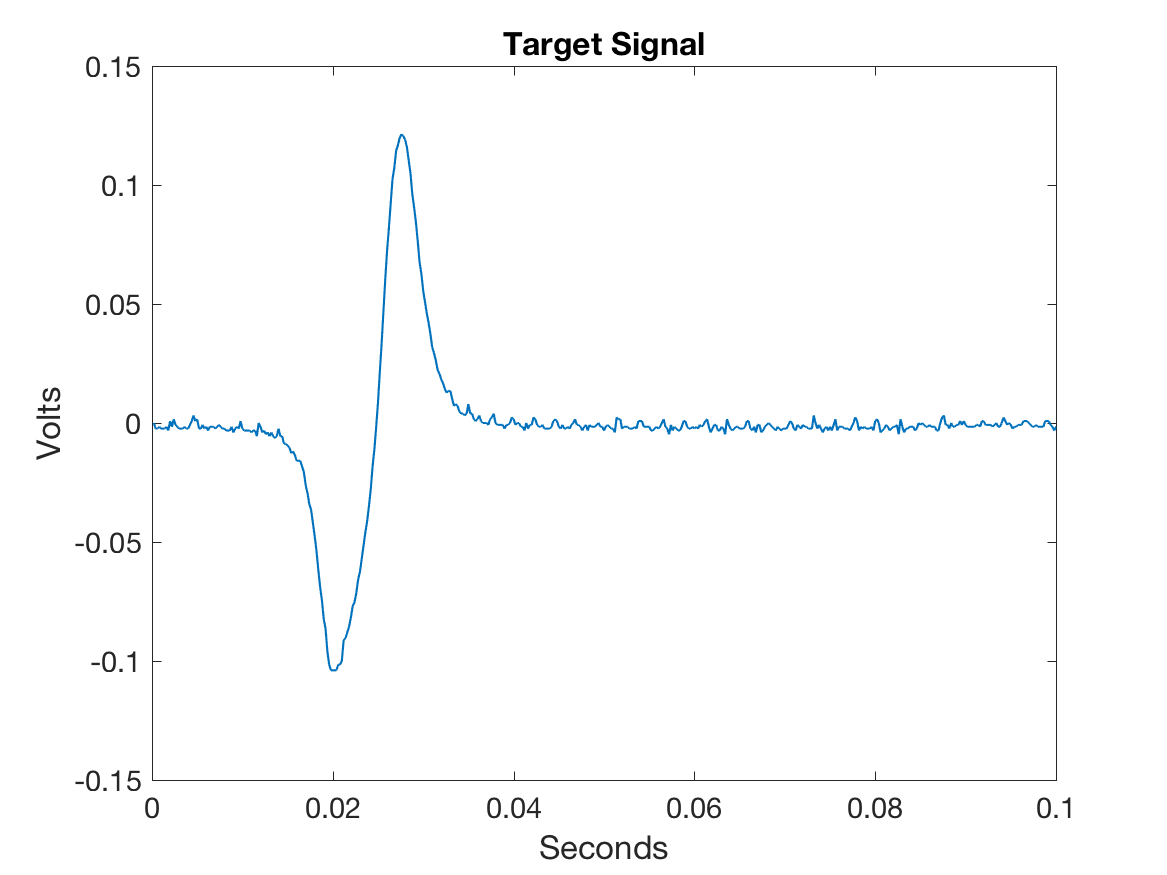
\includegraphics[width=8cm]{../matlab/plot5.png}
  \caption{Signal from prototype device}
  \label{fig:input}
  \end{figure}
Therefore we should
correlate our input signal with this signal to maximize the separation
from noise. To make sure this technique would suit our needs, a script
was created in MATLAB to illustrate the effects of the correlation.

First, the signal in Figure \,\ref{fig:input}. was modified by adding some noise, and appears in Figure \,\ref{fig:noisy}
\begin{figure}[h]
  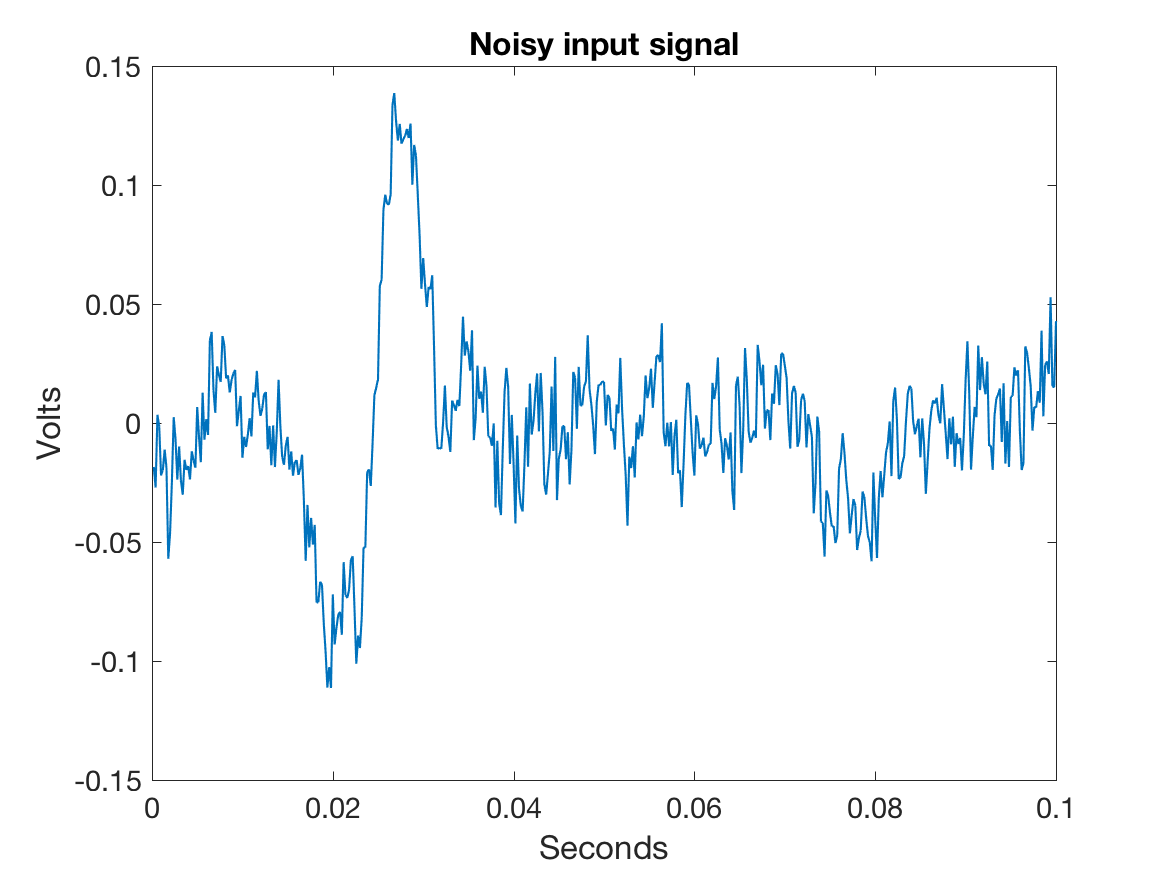
\includegraphics[width=8cm]{../matlab/plot1.png}
  \caption{Signal with simulated noise}
  \label{fig:noisy}
\end{figure}
Next, the signal was correlated with the signal in Figure \,\ref{fig:target}, and the resulting signal appears in Figure \,\ref{fig:correl}.

\begin{figure}[h]
  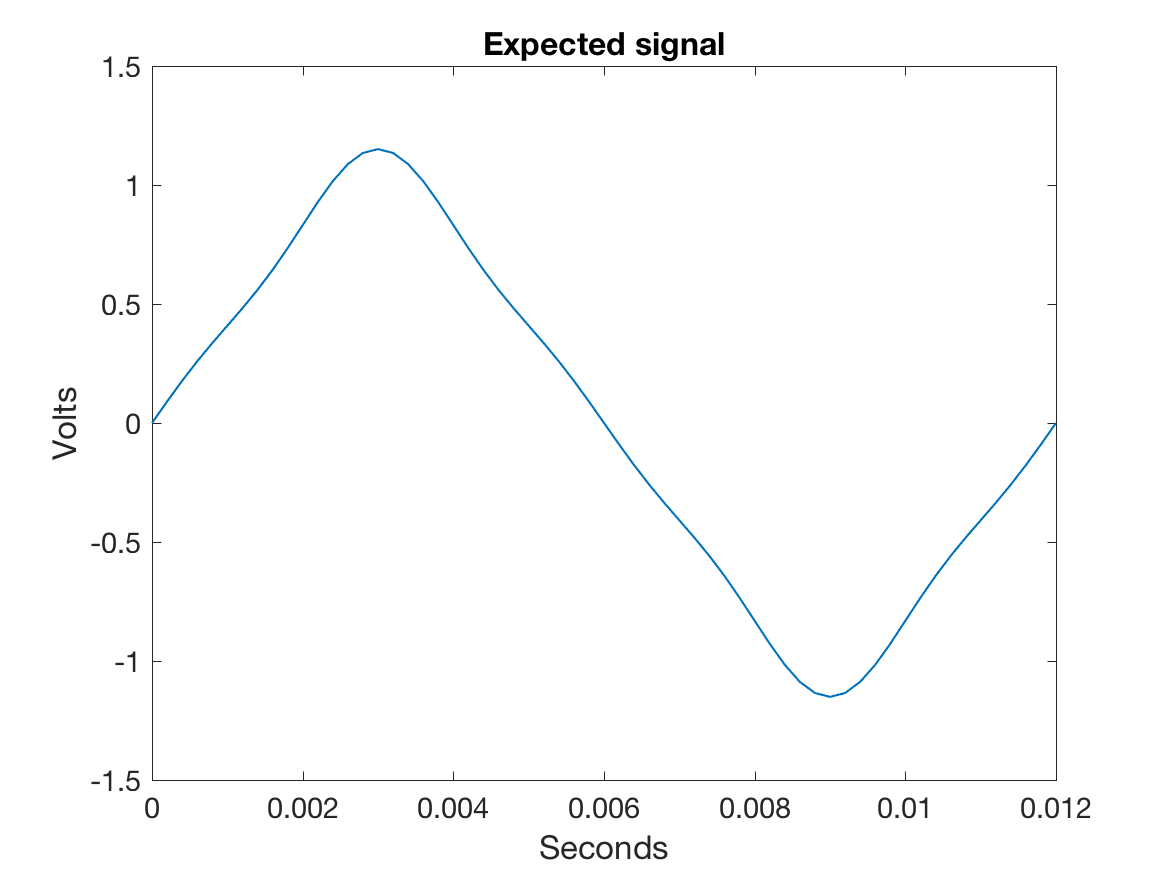
\includegraphics[width=8cm]{../matlab/plot2.png}
  \caption{Correlation target signal}
  \label{fig:target}
\end{figure}

\begin{figure}[h]
  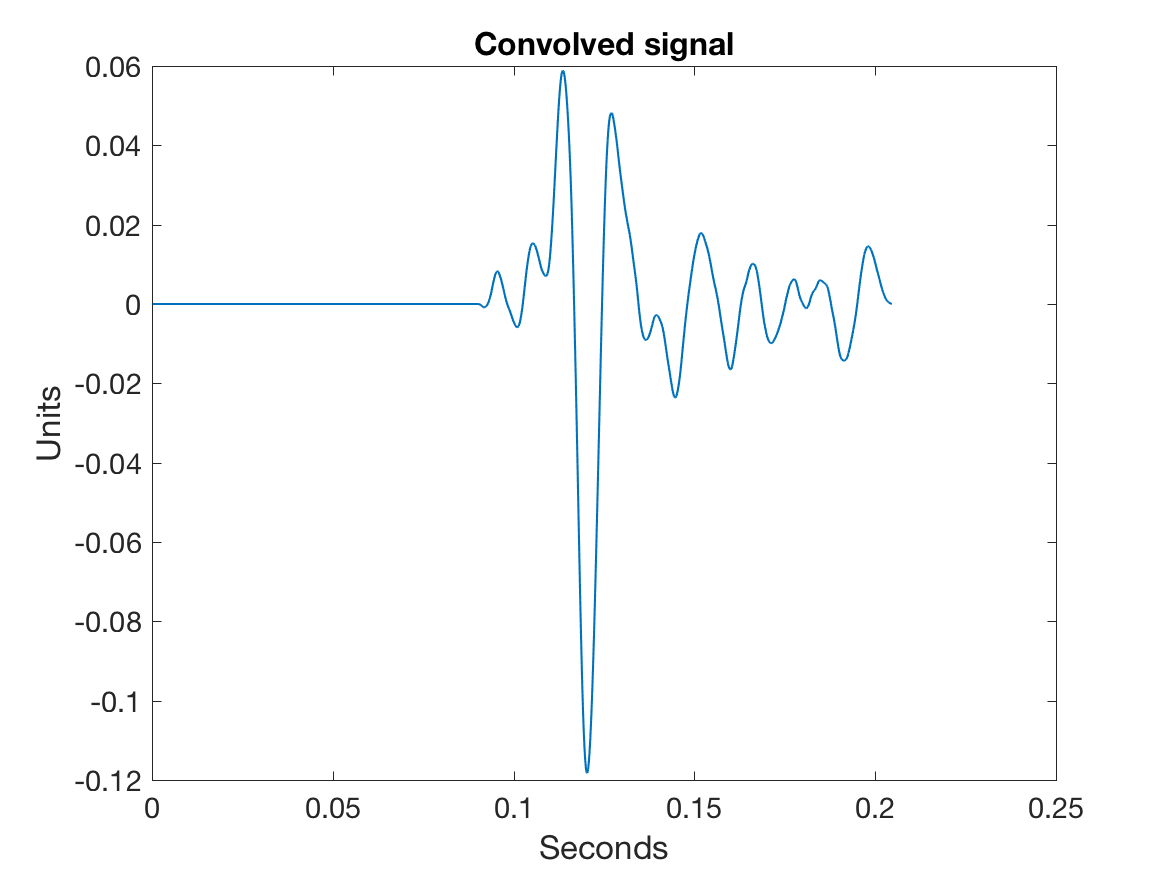
\includegraphics[width=8cm]{../matlab/plot3.png}
  \caption{Result of correlation}
  \label{fig:correl}
\end{figure}

Notice how Figure \,\ref{fig:correl} has several small bumps where the
target signal matched weakly with the noise, and also the very large
negative spike from where the target signal was lined up with the
pulse in the input signal. Unfortunately, the signal from the
uFluidics device can be either positive or negative, so further
processing is needed. To force both polarities to be positive, the
signal in Figure \,\ref{fig:correl} is squared, which also has the
effect of reducing the relative amplitude of the spikes from the noise
compared with the desired spike. Finally, the number of spikes above a
threshold value are counted, and the result appears in Figure
\,\ref{fig:result}.

\begin{figure}[h]
  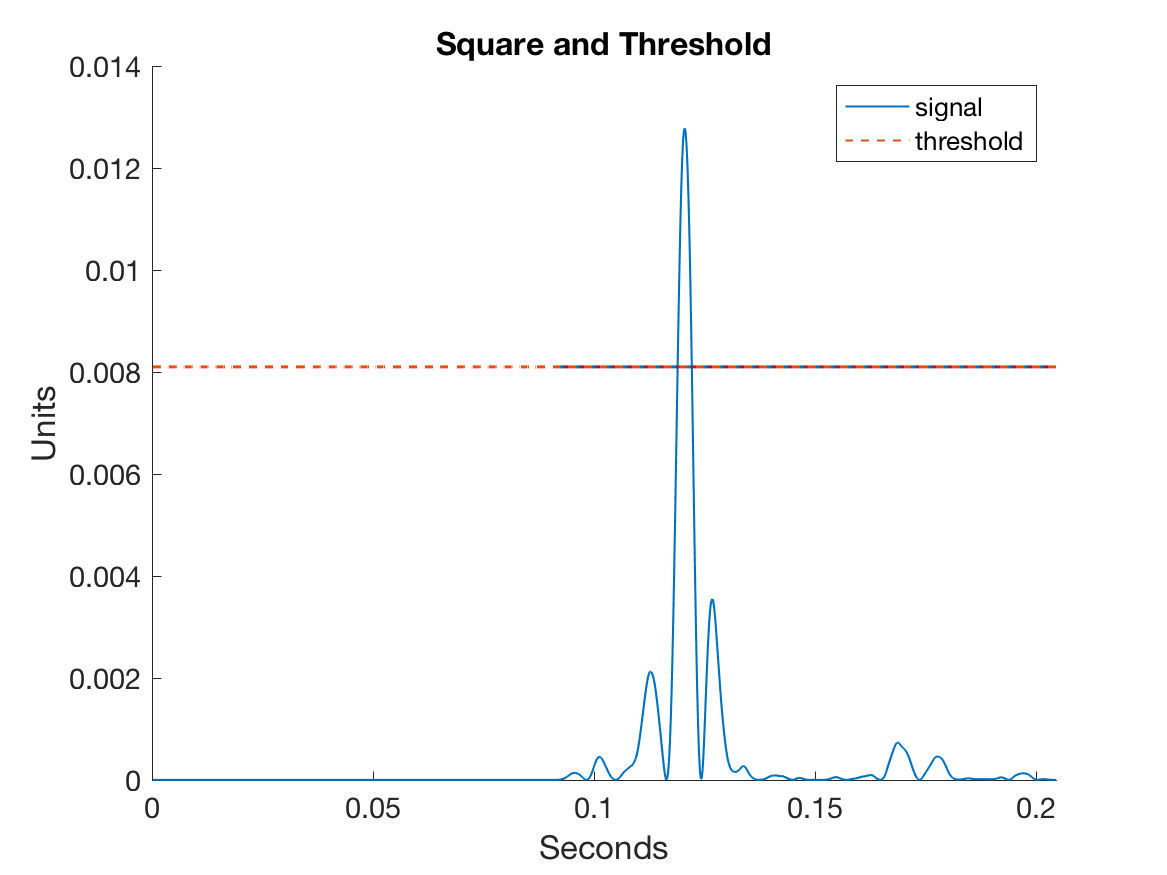
\includegraphics[width=8cm]{../matlab/plot4.png}
  \caption{Squared signal with threshold}
  \label{fig:result}
\end{figure}


\newpage
\bibliographystyle{ieeetr} \bibliography{dsp}{}

\end{document}
